% alfak2 sparse joint model, more than two time points: method B, state space
% (series = "state_space"). Mirrors sparse_joint_pair_left_out(),
% sparse_joint_pair_domains() and sparse_joint_state_space_problem() in
% R/sparse-joint-series-methods.R. Build: pdflatex flow_state_space.tex
\documentclass[tikz,border=4pt]{standalone}
% Shared style of the alfak2 flowcharts (doc/flowcharts/*.tex).
% Each chart is a standalone document; build one with
%   cd doc/flowcharts && pdflatex <chart>.tex
% or all of them with doc/flowcharts/build.sh. doc/alfak2_method.tex includes
% the PDFs.
\usepackage{amsmath,amssymb}
\usepackage[scaled=0.92]{helvet}
\renewcommand{\familydefault}{\sfdefault}
\usepackage{xcolor}
\usetikzlibrary{positioning,shapes.geometric,shapes.misc,arrows.meta,calc,fit,backgrounds}

% Thresholds of series = "auto" (sparse_joint_auto_thresholds in
% R/sparse-joint-series-methods.R). Change them here when the code changes.
\newcommand{\autoshare}{0.3}
\newcommand{\autoweight}{0.5}

\newcommand{\code}[1]{\texttt{\small #1}}

\definecolor{cIn}{HTML}{DCE6F2}    \definecolor{cInB}{HTML}{4F6D9A}
\definecolor{cProc}{HTML}{F5F5F5}  \definecolor{cProcB}{HTML}{707070}
\definecolor{cDec}{HTML}{FFF2CC}   \definecolor{cDecB}{HTML}{B8902B}
\definecolor{cTwo}{HTML}{D0E4F5}   \definecolor{cTwoB}{HTML}{2E6DA4}
\definecolor{cAnch}{HTML}{D9EAD3}  \definecolor{cAnchB}{HTML}{3D7A33}
\definecolor{cPair}{HTML}{FCE5CD}  \definecolor{cPairB}{HTML}{C0661A}
\definecolor{cState}{HTML}{E6DDF2} \definecolor{cStateB}{HTML}{6A4A9C}
\definecolor{cCore}{HTML}{EFEFEF}  \definecolor{cCoreB}{HTML}{8A8A8A}
\definecolor{cOut}{HTML}{D5EDEA}   \definecolor{cOutB}{HTML}{2C7C73}
\definecolor{cErr}{HTML}{F8D7D7}   \definecolor{cErrB}{HTML}{B03030}
\definecolor{cAuto}{HTML}{FFFBEA}

\tikzset{
  >={Stealth[length=2.4mm,width=1.8mm]},
  every node/.style={font=\small},
  box/.style={draw=#1B, fill=#1, rounded corners=2.5pt, line width=0.7pt, align=left,
              inner xsep=5pt, inner ysep=4pt},
  box/.default=cProc,
  w/.style={text width=#1},
  dec/.style={draw=cDecB, fill=cDec, chamfered rectangle, chamfered rectangle xsep=7pt,
              line width=0.7pt, align=center, inner xsep=3pt, inner ysep=3pt},
  err/.style={box=cErr, font=\footnotesize},
  tag/.style={draw=#1, dashed, rounded corners=6pt, fill=white, font=\scriptsize, inner sep=2.5pt,
              align=center},
  arr/.style={->, line width=0.8pt, draw=black!75},
  darr/.style={->, line width=0.8pt, draw=black!60, dashed},
  lab/.style={font=\footnotesize\itshape, fill=white, inner sep=1.5pt, text=black!85},
  frame/.style={draw=#1, rounded corners=6pt, line width=0.9pt, inner sep=7pt},
  ftitle/.style={font=\footnotesize\bfseries, fill=white, inner sep=2pt, text=#1},
}

\begin{document}
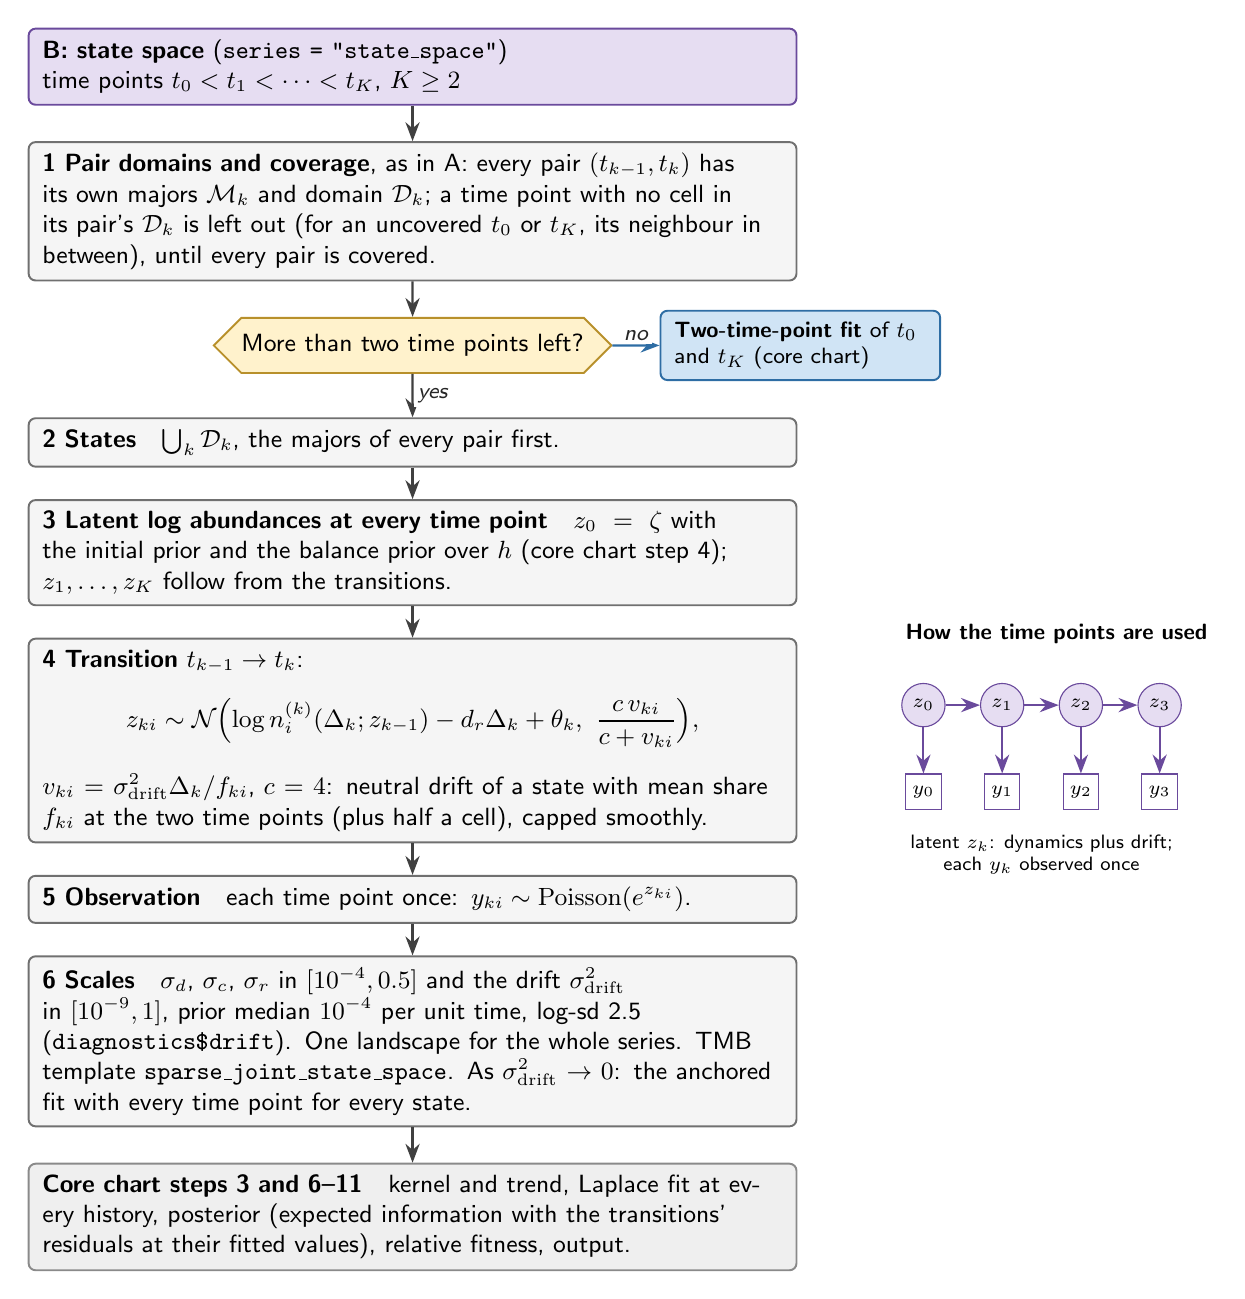
\begin{tikzpicture}

\node[box=cState, w=9.4cm] (in) at (0,0) {%
  \textbf{B: state space} (\code{series = "state\_space"})\\
  time points $t_0<t_1<\dots<t_K$, $K\ge2$};

\node[box, w=9.4cm, below=0.45cm of in] (pairs) {%
  \textbf{1 Pair domains and coverage}, as in A: every pair $(t_{k-1},t_k)$ has its own majors
  $\mathcal M_k$ and domain $\mathcal D_k$; a time point with no cell in its pair's $\mathcal D_k$ is left
  out (for an uncovered $t_0$ or $t_K$, its neighbour in between), until every pair is covered.};
\node[dec, below=0.45cm of pairs] (two) {More than two time points left?};
\node[box=cTwo, w=3.2cm, font=\footnotesize, right=0.6cm of two] (twofit) {%
  \textbf{Two-time-point fit} of $t_0$ and $t_K$ (core chart)};
\draw[arr] (in) -- (pairs);
\draw[arr] (pairs) -- (two);
\draw[arr, draw=cTwoB] (two) -- node[lab, above] {no} (twofit);

\node[box, w=9.4cm, below=0.55cm of two] (states) {%
  \textbf{2 States}\quad $\bigcup_k\mathcal D_k$, the majors of every pair first.};
\draw[arr] (two) -- node[lab, right] {yes} (states);

\node[box, w=9.4cm, below=0.4cm of states] (latent) {%
  \textbf{3 Latent log abundances at every time point}\quad $z_0=\zeta$ with the initial prior and the
  balance prior over $h$ (core chart step 4); $z_1,\dots,z_K$ follow from the transitions.};
\node[box, w=9.4cm, below=0.4cm of latent] (trans) {%
  \textbf{4 Transition} $t_{k-1}\to t_k$:
  \[z_{ki}\sim\mathcal N\Bigl(\log n^{(k)}_i(\Delta_k;z_{k-1})-d_r\Delta_k+\theta_k,\ \frac{c\,v_{ki}}{c+v_{ki}}\Bigr),\]
  $v_{ki}=\sigma^2_{\mathrm{drift}}\Delta_k/f_{ki}$, $c=4$: neutral drift of a state with mean share
  $f_{ki}$ at the two time points (plus half a cell), capped smoothly.};
\node[box, w=9.4cm, below=0.4cm of trans] (obs) {%
  \textbf{5 Observation}\quad each time point once: $y_{ki}\sim\mathrm{Poisson}(e^{z_{ki}})$.};
\node[box, w=9.4cm, below=0.4cm of obs] (scales) {%
  \textbf{6 Scales}\quad $\sigma_d$, $\sigma_c$, $\sigma_r$ in $[10^{-4},0.5]$ and the drift
  $\sigma^2_{\mathrm{drift}}$ in $[10^{-9},1]$, prior median $10^{-4}$ per unit time, log-sd 2.5
  (\code{diagnostics\$drift}). One landscape for the whole series. TMB template
  \code{sparse\_joint\_state\_space}. As $\sigma^2_{\mathrm{drift}}\to0$: the anchored fit with every
  time point for every state.};
\draw[arr] (states) -- (latent);
\draw[arr] (latent) -- (trans);
\draw[arr] (trans) -- (obs);
\draw[arr] (obs) -- (scales);

\node[box=cCore, w=9.4cm, below=0.45cm of scales] (core) {%
  \textbf{Core chart steps 3 and 6--11}\quad kernel and trend, Laplace fit at every history, posterior
  (expected information with the transitions' residuals at their fitted values), relative fitness,
  output.};
\draw[arr] (scales) -- (core);

% ---- schematic --------------------------------------------------------------
\begin{scope}[shift={($(trans.east)+(2.6,0.1)$)}]
  \node[font=\footnotesize\bfseries, anchor=west] at (-1.35,1.25) {How the time points are used};
  \foreach \k/\x in {0/-1.0, 1/0.0, 2/1.0, 3/2.0} {
    \node[circle, draw=cStateB, fill=cState, minimum size=5.5mm, inner sep=0pt, font=\scriptsize] (z\k) at (\x,0.35) {$z_\k$};
    \node[rectangle, draw=cStateB, fill=white, minimum size=4.5mm, inner sep=0pt, font=\scriptsize] (y\k) at (\x,-0.75) {$y_\k$};
    \draw[->, cStateB, line width=0.7pt] (z\k) -- (y\k);
  }
  \foreach \a/\b in {z0/z1, z1/z2, z2/z3} {
    \draw[->, cStateB, line width=0.8pt] (\a) -- (\b);
  }
  \node[font=\scriptsize, align=center] at (0.5,-1.55) {latent $z_k$: dynamics plus drift;\\
    each $y_k$ observed once};
\end{scope}

\end{tikzpicture}
\end{document}
